%% LaTeX2e class for seminar theses
%% sections/content.tex
%% 
%% Karlsruhe Institute of Technology
%% Institute for Program Structures and Data Organization
%% Chair for Software Design and Quality (SDQ)
%%
%% Dr.-Ing. Erik Burger
%% burger@kit.edu
%%
%% Version 1.0, 2018-04-16

\section{Basics}
\label{ch:Basics}

In this chapter the basics needed to understand the changes made in SegWit are being explained. These consist of the way a transaction is built (\autoref{sec:Basics:Transaction}), a short explanation of merkle trees and their use (\autoref{sec:Basics:MerkleTree}), and the problems of bitcoin being the current Blocksize limit (\autoref{sec:Basics:BlocksizeLimit}) and Transaction Malleability (\autoref{sec:Basics:TransactionMalleability}). If you already know these basics you can of course skip straight to the SegWit changes (\autoref{ch:SegWit}).

\subsection{Transaction}
\label{sec:Basics:Transaction}

\begin{figure}[!ht]
    \centering
    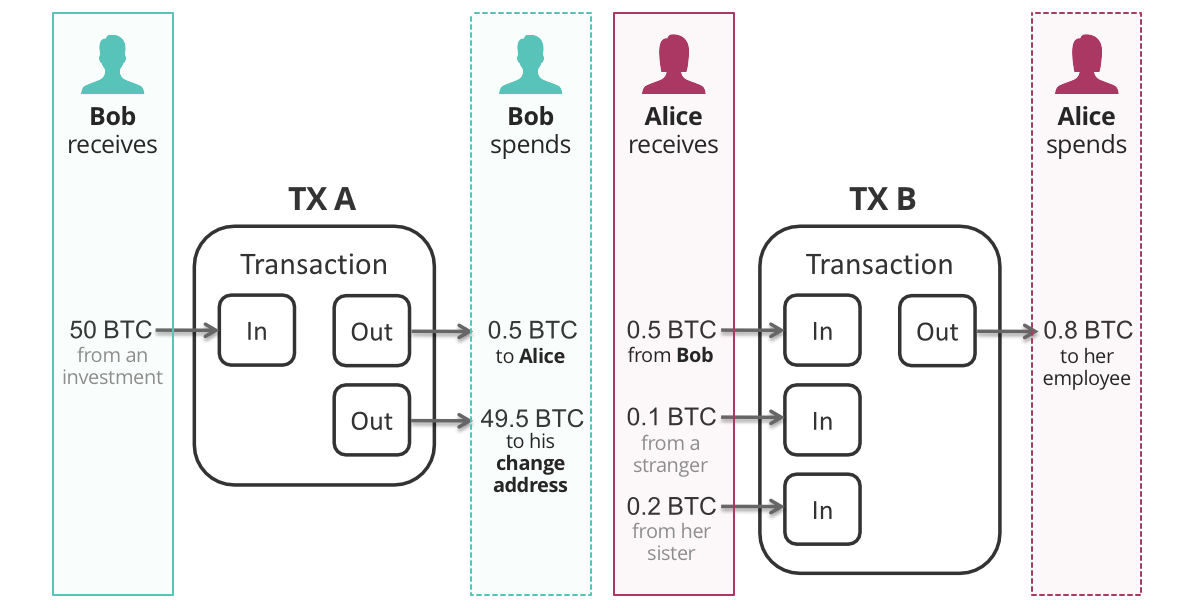
\includegraphics[width=(\textwidth * 2 / 3 )]{Ausarbeitung/images/transaction.png} \caption[Transaction]{Transaction}
    \small \url{https://thecoinrise.com/wp-content/uploads/2019/08/how-do-bitcoin-transaction-work.png}
    \label{fig:transaction}
\end{figure}
Every transaction is built up with a version number, transaction inputs, transaction outputs and a lock time.
The version number just defines which version is used in this transaction. This can be differently for different transactions.
The lock time describes when the transaction should be seen as final. Either it is empty and it should be seen as final on publication, or it has a block height or timestamp as an argument, which tells when the transaction is final.
The first transaction in any block is called "coinbase" transaction and just credits a fix amount of bitcoins plus the sum of all transaction fees in the block. The transaction fees aggregate when the inputs of a transaction contain more bitcoin than the outputs.
Every transaction in any block must have at least one input and at least one output. In \autoref{fig:transaction} Tx A has on Input and two outputs an Tx B has three inputs and one output. The inputs must, except in the "coinbase" transaction, refer to an output of a previous transaction which was not spent yet, called an unspent transaction output or UTXO. For example the first input of Tx B in \autoref{fig:transaction} refers to the first output of Tx A, which is just spent in Tx B.
Finally the transaction has to be signed. There are multiple ways to do this, but the signature is always, before SegWit, contained partly inside the inputs and partly inside the outputs.

\subsubsection{Transaction ID}
To broadcast a transaction into the Bitcoin network it has to be serialized first. Using this serialized data a Transaction ID, or TXID, is calculated for every transaction. This is done by applying double SHA-256 on the serialized data and the resulting hash is then used as the ID for this transaction.


\subsection{Merkle Tree}
\label{sec:Basics:MerkleTree}
\begin{figure}[!ht]
    \centering
    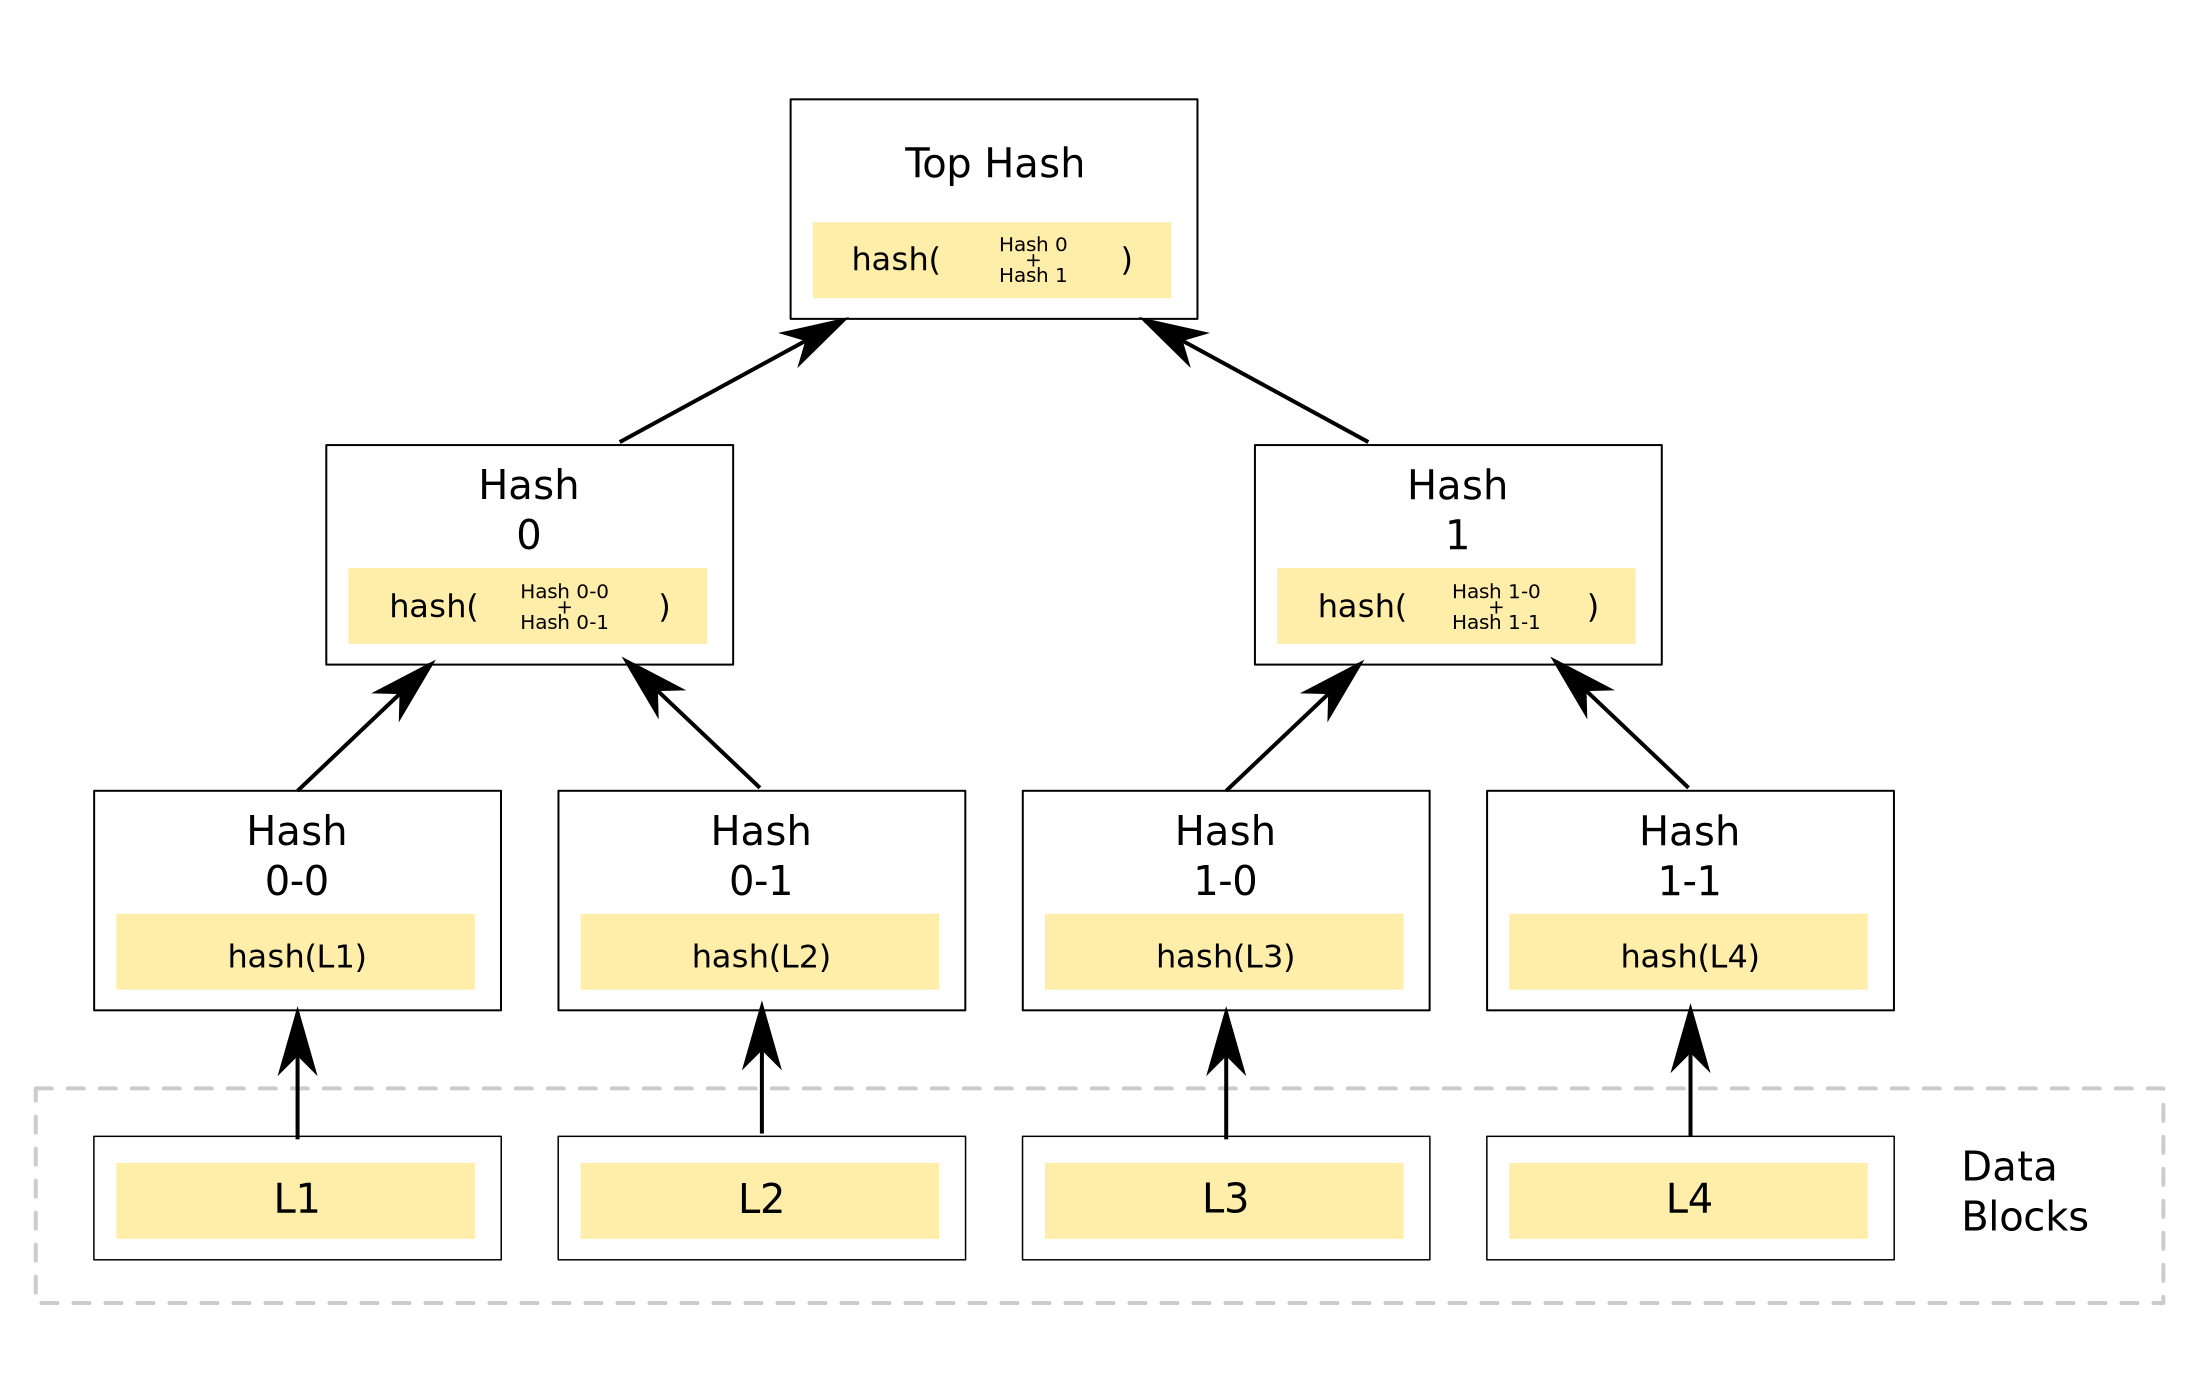
\includegraphics[width=(\textwidth * 2 / 3 )]{Ausarbeitung/images/merkle_tree.png}
    \caption[Merkle Tree]{Merkle Tree}
    \small \url{https://en.wikipedia.org/wiki/Merkle_tree#/media/File:Hash_Tree.svg} 
    \label{fig:merkle_tree}
\end{figure}
A merkle tree, or binary hash tree as shown in \autoref{fig:merkle_tree} is a tree where all the leaves, in the case of bitcoin the leaves are the transactions of a block, are concatenated and then hashed pairwise. This results in a new layer of nodes, which are then again concatenated and then hashed pairwise until there is only one node left, called the merkle root. In \autoref{fig:merkle_tree} the merkle root is called "top hash", while L1 through L4 represent the leaves and thus transactions of the corresponding block. \\



\subsection{Blocksize limit}
\label{sec:Basics:BlocksizeLimit}
Before SegWit blocks were "limited to 1,000,000 bytes (1MB) total size" \cite{bip-141}. This and the fact that there is only supposed to be one new block ever ten minutes \cite{nakamoto} results in a limit of about 4.6 transactions per second\footnote{can be seen on \url{https://www.blockchain.com/charts/transactions-per-second}}\cite{hackernoon}. Compared to Visa's 1,700 transactions per second \cite{hackernoon} it is obvious that at this state Bitcoin cannot work on a large scale as it simply cannot handle enough transactions.



\subsection{Transaction Malleability}
\label{sec:Basics:TransactionMalleability}
Since the Transaction ID is calculated by hashing the serialized data of a transaction it is influenced by the signature. There is a problem with this where an attacker can change the whole Transaction ID by changing the unlocking script in a way that does not change the way it works. For example he can just zero pad some data being used which does not change the functionality but very much changes the resulting hash. \\

\subsubsection{Example of a Malleability attack}
\label{subsec:Basics:TransactionMalleability:Attack}
In this example Alice is the victim and Bob is the attacker. \\
Alice sends a transaction worth one bitcoin to Bob with Transaction ID A.
Bob now alters the Transaction ID abusing Transaction Malleability and broadcasts the same transaction but with the now different Transaction ID B.
Now Bob is lucky as the transaction with ID B is confirmed before the one with ID A is. Since the UTXO used as input in both transactions is the same, the transaction with Transaction ID A is being declined.
Now Bob, who has received one bitcoin, informs Alice that he has not received the transaction. After Alice checks that no transaction with Transaction ID A got accepted in any block she assumes it must have failed.
Now Alice sends the transaction again resulting in a double spend where Bob receives two bitcoin instead of one.

\subsubsection{Mt.Gox}
One of the biggest bitcoin exchange points ever, which in February 2014 "still accounted for close to 70\% of all bitcoins ever traded" \cite{springer:malleability_and_mtgox}, had to file for bankruptcy in the same month resulting in "the loss of over 500 million USD worth of bitcoins owned by its customers" \cite{springer:malleability_and_mtgox}. \\
Later they stated that the main cause for this was Transaction Malleability \cite{springer:malleability_and_mtgox}.

\subsection{Soft Fork}
\label{sec:Basics:SoftFork}
To prevent a spl


\section{Segregated Witness}
\label{ch:SegWit}
\todo{description of what segwit is}


\subsection{Idea}
\label{sec:SegWit:Idea}
To solve the problem of Transaction Malleability the signature and unlocking script are moved into a new data structure called "witness". This way the signature will no longer effect the identification of a transaction, fixing the problem of Transaction Malleability. This new structure has its own ID called WTXID or Witness Transaction Identifier. The separation of witness data from transaction data makes the transmission of the signature data optional, as it is only used for verification of a transaction and not needed for checking its existence. \\
Additionaly it is implemented in such a way that it is backwards compatible, meaning older versions of the Bitcoin protocol are still compatible with these new changes, and can be published as a soft fork \todo{maybe explain here}, taking away the downside of splitting the network in two. This can be accomplished even though there are many changes made, including an upgrade of the block size limit up to theoretical four megabytes. Also Segregated Witness introduces a new commitment structure making future updates simpler. \\
Finally the fix of Transaction Malleability "allows creation of unconfirmed transaction dependency chains without counterparty risk"\cite{bip-141} like the Lightning network, providing Bitcoin to be a tool for everyday transactions. This has the potential to not only fix Transaction Malleability, but also move a big step to solve the Scalability Problem.


\subsection{Implementation}
\label{sec:SegWit:Implementation}

\todo{changes to transaction ID, witness programs functionality and script semantics, other consensus critical limits, additional definitions, commitment structure, extensible commitment structure, Backward compatibility}





\subsection{Consequences}
\label{sec:SegWit:Consequences}

\todo{Fixes transaction malleability, increases blocksize limit to an extent -> no solution but rather a slight improvement}

\subsection{Future possibilities}
\label{sec:SegWit:Future}
\todo{Trust-free unconfirmed transaction dependency chain (Lightning Network), Future extensions}

\subsection{History of Segregated Witness}
\label{sec:SegWit:History}

\todo{find good source for this}

%\subsection{Trial of SegWit2x}